\documentclass{article}
\usepackage[utf8]{inputenc}

\title{PS6Buchman}
\author{blakebuchman03 }
\date{March 2021}

\usepackage{natbib}
\usepackage{graphicx}

\begin{document}

\maketitle

\section{Cleaning the Data}
The only thing I had to do to clean the data was to take out columns 10-22 because they were not needed for what I wanted to convey. 
\section{Image Explanations}
Image a shows the relationship between adjusted offensive efficiency and team wins overall. This is important because while it may seem obvious, it is easy to see the correlation in a visualization. 
\newline
\newline Image b shows a smooth line of the relationship between effective offensive FG percentage and team wins. Once again, seeing a visualization makes this easier to understand and you see the relationship clearly. 
\newline
\newline Image c shows the count of teams with each value for adjusted defensive efficiency. This is important because it will show you where your team lies as far as the average for the rest of the country.


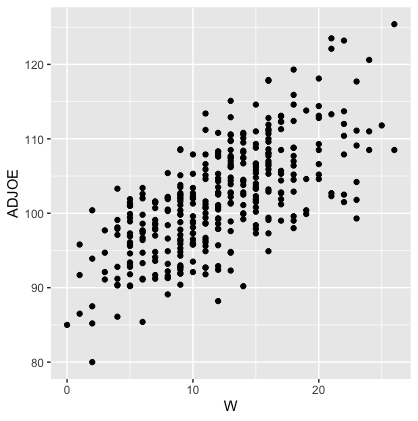
\includegraphics{PS6a_Buchman}
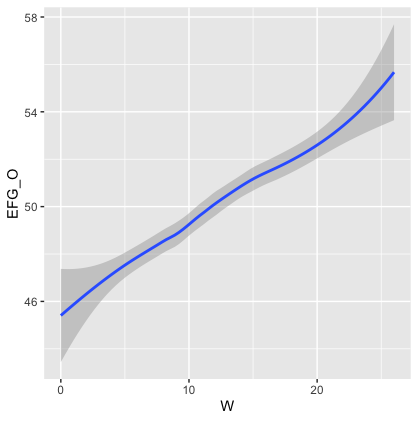
\includegraphics{PS6b_Buchman.png}
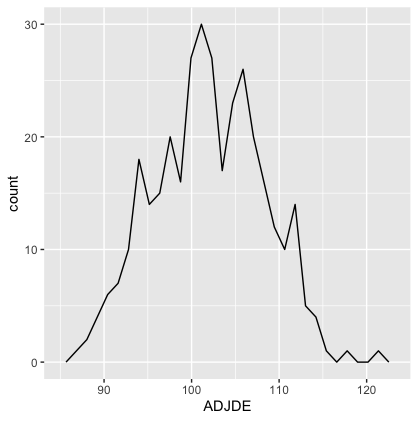
\includegraphics{PS6c_Buchman.png}
\centering

\end{document}
